\section{Erweiterung}
\subsection{Grunds"atzliches}
Eine Extentsion f"ur NetLogo ist nichts anderes als ein Jar-Archiv. Die Erweiterung
muss in einem Unterverzeichnis des Models, welches die Erweiterung verwenden will,
oder in einem Unterverzeichnis des NetLogo-Programmes liegen. Jede Extension
ben"otigt einen ClassManager. Dieser teilt NetLogo mit welche Befehle die 
Erweiterung mit sich bringen wird. 
\lstset{language=Java} Jeder dieser Befehle ist von \lstinline|org.nlogo.api.Primitive|
abgeleitet. Die Erweiterung muss zus"atzlich ein Manifest mit den folgenden 
Befehlen enthalten (am Beispiel meiner Erweiterung):
\begin{verbatim}
Manifest-Version: 1.0
Extension-Name: midi
Class-Manager: at.univie.csd.MidiManager
NetLogo-Extension-API-Version: 4.1
\end{verbatim}

\subsection{Unterlagen}
F"ur die Erstellung der Erweiterung wurden im wesentlich folgende Quellen 
zu Theorie zu Midi zur Rate gezogen: \cite{midi-inst}, \cite{midi-java} und
\cite{midi-javafaq} verwendet. 


\subsection{Struktur}
\begin{figure}[hbt]
	\centering
		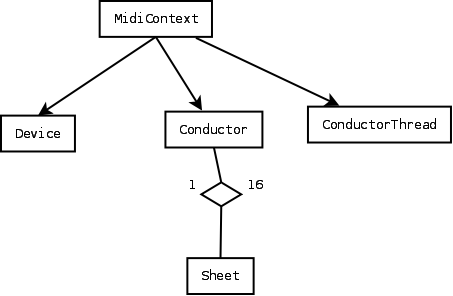
\includegraphics[scale=0.5]{fig/struktur.png}
	\caption{Struktur}
	\label{fig:struktur}
\end{figure}
Die Erweiterung besitzt eine relativ einfache Struktur. Beim laden der Erweiterung
wird eine \lstinline|MidiContext| Instanz erzeugt. Um eine Synchronisation der
Zugriffe auf die Objekte zu erm"oglichen habe ich in Anlehnung an \cite{fh-wedel} 
einfache Semaphore implementiert. Anstatt von Integerz"ahlern habe ich einfach
boolesche Variablen verwendet. Bei den Tests hat dies zu keinen Problemen gef"uhrt.
Zu finden sind die Semaphore in der Klasse MidiContext in der Datei 
''MidiContext.java''. 

Die Implementierung als Semaphor mit Z"ahler w"urde wie folgt aussehen:
\begin{lstlisting}[language=Java,basicstyle=\small]
	...
	private int m_free = 1;
	...
	public synchronized MidiDevice getDevice()
	{
		while( m_free <= 0 )
		{
			try
			{
				wait();
			}
			catch(InterruptedException e)
			{
			}
		}
		m_free--;
	}
	...
	public synchronized void releaseDevice()
	{
		m_free++;
		notify();
	}
\end{lstlisting}
Analog die Impelentierung f"ur den Conductor-Semaphor. 
\subsubsection{MidiContext}
Der MidiContext soll sich um die Synchronisation der Threads k"ummern. Da nur
ein Device zum abspielen der MidiBefehle ge"offnet wird muss der Zugriff 
synchronisiert werden. Um einen Befehl schreiben zu k"onnen muss zuerst der
Zugriff reserviert werden. Dies geschieht "uber den Befehl
\lstinline|MidiManager.getMidiContext().getDevice();|. Nat"urlich muss auch noch
"uberpr"uft werden ob das Device auch offen ist. Um das Device wieder f"ur andere
Threads wieder frei zu geben muss der Befehl
\lstinline|MidiManager.getMidiContext().releaseDevice();| verwendet werden. 

\subsubsection{Conductor}
Weiters beinhaltet der MidiContext eine Instanz des Conductors. Diese Klasse 
soll helfen einen virtuellen Dirigenten zu erstellen. Dazu hat die Klasse 
bis zu 16 Notenbl"atter. Die Anzahl ist Aufgrund der Midi-Spezifikation von
16 Kan"alen festgesetzt worden. Auch hier muss wieder um die Synchronit"at 
zugew"ahrleisten mit den Befehlen \lstinline|MidiManager.getMidiContext().getConductor();|
und \lstinline|MidiManager.getMidiContext().releaseConductor();| gearbeitet 
werden. 

\subsubsection{Sheet}
Die Klasse Sheet hilft bei der Verwaltung von Kommandos, die timecode gesteuert
ausgef"uhrt werden sollen. Sheet ist das Pendant zu Streams in MidiCSD \cite{MidiCSD}
Jedes Notenblatt verf"ugt "uber eine Liste von Kommandos. Zu Begin der Arbeit
war die Anzahl dieser Commandos auf die des MidiCSD-Toolkits beschr"ankt und 
jeder dieser Befehle wurde intern zu den entsprechenden Midi-Befehlen kompiliert.
Dies wurde jedoch in R"ucksprache und auf Wunsch des Betreuers so ge"andert, 
dass nun jedes beliebige Kommando hinzugef"ugt werden kann. W"ahrend des
Programmablaufes wird also das Kommando nur gespeichert und dann NetLogo zur
Ausf"uhrung "ubergeben. Dies f"uhrt zu kleinen Laufzeiteinbusen, erh"oht jedoch
aber die Flexibilit"at und erweitert die M"oglichkeiten f"ur den Einsatz der 
Erweiterung. So ist es zum Beispiel m"oglich den virtuellen Musikern nicht nur
Noten sondern auch Bewegungen beizubringen. 
Der ''alte'' Code wurde als Kommentar im Source-Code hinterlassen. 

\subsubsection{ConductorThread}
Damit der Dirigent im Hintergrund die Notenbl"atter abarbeiten kann, wurde der
CondutorThread erstellt. Dieser, wenn gestartet, arbeitet St"uck f"ur St"uck
die Notenbl"atter ab. Dies macht er, in dem er sich in jedem Schritt einen
Zugriff auf den Conductor reserviert um sich die anstehenden Kommandos zu besorgen.
Diese werden dann sequentiell ausgef"uhrt. Danach legt sich der ConductorThread
f"ur 100ms schlafen um den anderen Threads nicht im Weg zu stehen. 

\subsection{Neue Befehle}
Um einfach neue Midi-Befehle implementieren zu k"onnen habe ich eine Klasse
\lstinline|MidiCommand| geschrieben. Diese besitzt im wesentlichen zwei 
Methoden: \lstinline|preAction| und \lstinline|postAction|. Jeder neue Midi-Befehl,
wenn von dieser Klasse abgeleitet, kann sich \lstinline|preAction| Zugriff auf
das Midi-Device holen und diesen dann wieder mit \lstinline|postAction| freigeben.
So kann sicher gestellt werden, dass durch neue Befehle kein Wirrwarr von offenen
Devices entsteht. Weiters erh"oht diese Vorgangsweise die Modularit"at. Soll zum
Beispiel etwas an der Art wie das Device ge"offnet wird ge"andert werden, muss
dies nur an einer Stelle angepasst werden. 


